%time error analysis
%ss 

\section{Muon Time Error Analysis}\label{muontimeerroranalysis}

The main source of statistical error for $\tau_{\mu}$ was due to the fitting process.  Using 2-parameter nonlinear regression, the data in Figure \ref{fig:muondecay} is approximated by

\begin{equation}
\label{nonlinfit}
y_{i}=f(\mathbf{\beta},\mathbf{x_{i}'})+\epsilon_{i}
\end{equation}

where $y_{i}$ is the $i$th expected value, $\mathbf{\beta}$ is a parameter vector, $\mathbf{x_{i}'}$ is the $i$th row of predictors, and $\epsilon_{i}$ is the associated random error.  The Likelihood, $L$, is given by 

\begin{equation}
\label{likelihood}
L(\beta,\sigma^{2})=\frac{1}{(2\pi\sigma^{2})^{n/2}}exp(-\frac{\sum_{i=1}^{n}[y_{i}-f(\beta,\mathbf{x_{i}'})]^{2}}{2\sigma^{2}})
\end{equation}

where $n$ is the number of data points and $\sigma^{2}$ is the variance. $L$ is maximized where the sum of squared errors, $S(\beta)$, given by

\begin{equation}
\label{sse}
S(\beta) = \sum_{i=1}^{n}[y_{i}-f(\mathbf{\beta},\mathbf{x_{i}'})],
\end{equation}

is minimized.  Furthermore, each data point was weighted by $\sqrt{N_{\mu}}$, where $N_{\mu}$ was the number of muons with some measured lifetime.  The optimal choice for parameters with weightings yields a statistical error of $2.8\%$.  

An additional source of statistical error is the jitter in the electronics.  However because the number of events is so large ($N=14,632$), the contribution of the total jitter to the total error is on the order of single nanoseconds.  This is more precise than our actual measurement of $\tau_{\mu}$ and is thus disregarded. 
 
Systematic error was also added to the total error.  PMT false flashes served as a main source of systematic error.  As discussed in Section \ref{autocorrelator}, autocorrelated events were measured by an autocorrelator. These false flashes were found to die off approximately exponentially on the order of $\tau_{\mu}$ as seen in Figure \ref{fig:autocorr}.  Because of this, we expect the data shown in Figure~\ref{fig:muondecay} to be slightly corrupted and generally skewed in a specific direction for small $t$.  This distortion will affect the calculated value for $\tau_{\mu}$.  To account for this skew we attributed $5\%$ systematic error to $\tau_{\mu}$.

\begin{figure}[h]
\begin{center}
\subfigure[Bottom detector]{\label{fig:edge-a}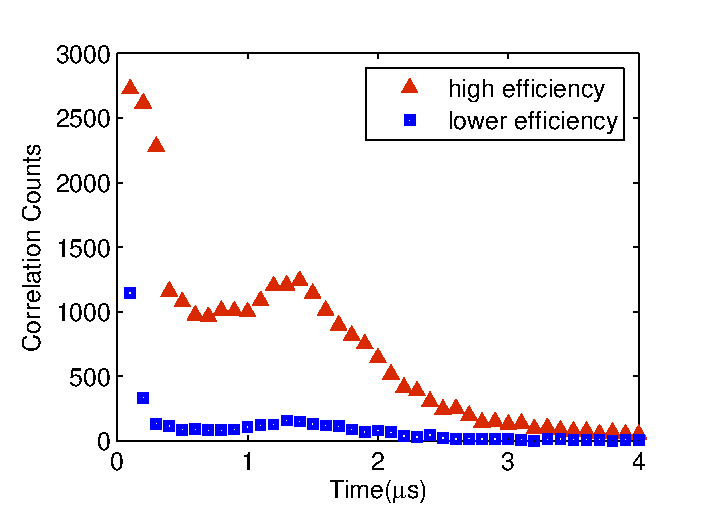
\includegraphics[width=0.5\textwidth]{figures/Bcorr.eps}}
\hspace{-7mm}
\vspace{-2mm}
\subfigure[Middle detector]{\label{fig:edge-b}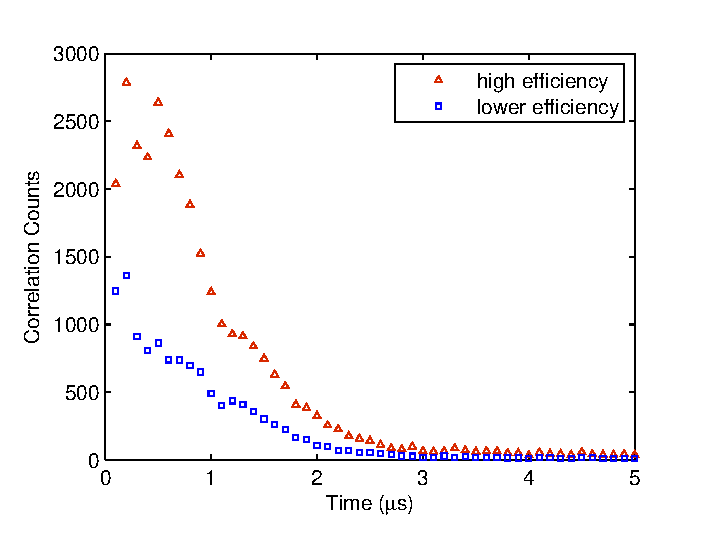
\includegraphics[width=0.5\textwidth]{figures/Mcorr.eps}}
\vspace{-2mm}
\subfigure[Top detector]{\label{fig:edge-c}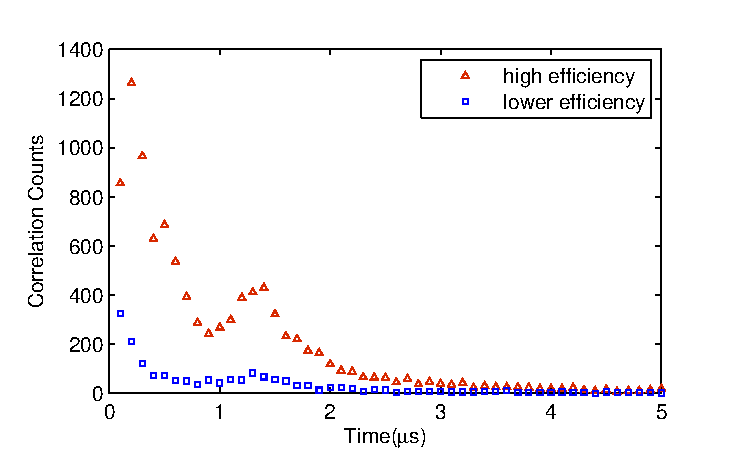
\includegraphics[width=0.5\textwidth]{figures/Tcorr.eps}}
\vspace{-2mm}
\caption{These plots show the existence of autocorrelated events, or false flashes, produced by the PMTs.  These events occur most frequently immediately after a true scintillator flash and decrease as $t$ increases.  The overall amount of autocorrelated events was decreased by increasing the discriminator threshold from $70mV$ to $100 mV$, which, however, decreased the relative efficiency of the detectors.}
\label{fig:autocorr}
\end{center}
\end{figure}

Another source of systematic error in the time measurement was due to the proton capture of muons given by Equation \eqref{pcap}.  As discussed in Section \ref{decayinmatter}, this decay has a mean lifetime on the order, but slightly less, than the muon decay we are concerned with.  As a result we would expect our data, shown in Figure \ref{fig:muondecay}, to be modeled by the summation of two linearly independent exponentials above some noise floor given by

\begin{center}
\begin{equation}
\label{eq:2decay}
N(t)=N_{0}(r e^{-t/\tau_{\mu}}+(1-r)e^{-t/\tau_{\mu p}})
\end{equation}
\end{center}

where $r$ is some relative weighting between the two decays which is determined by the material in which the decay occurs.  As stated in Section \ref{decayinmatter}, the expected mean lifetime for the proton capture of a muon would lie between $1.5 \mu s$ and $1.9 \mu s$.  Fitting to Equation \eqref{eq:2decay} gives a greater value for $\tau_{\mu}$.  However due the effects of autocorrelation, the relative uncertainty of the $r$, and the dependency of $\tau_{\mu p}$ on the material, a better fit (relative to the fit produced using the procedure described in Section \ref{determinationofmuonlifetime}) was not able to be produced.  As a result, we determined that attributing $5\%$ systematic error to $\tau_{\mu}$ was sufficient to account for any effect that proton capture had on the data. 

Another possible source of systematic error would be due to systematic shifts in pulse lengths or pulse delays.  This systematic error, which is most likely present, causes lifetime values to be shifted in a certain direction.  However because the data assumes an exponential decay shown in Figure \ref{fig:muondecay}, this time offset would not affect the overall mean lifetime, $\tau_{\mu}$, but would only affect the coefficient.  Therefore we are not concerned with this type of systematic error.

Ultimately, our total statistical error is due to the error in our fit which is $2.8\%$.  Our total systematic error comes from both the PMT false flashes and the effect of proton capture.  These errors added in quadrature are calculated to be $7\%$.  With this error included, we calculate the muon mean lifetime to be $2.12\pm.06$ (statistical) $\pm.15$ (systematic) $\mu s$.  Added in quadrature $\tau_{\mu}=2.12\pm.16\mu$.
